\documentclass[a4paper,11pt,fleqn]{scrartcl}%fleqn pour aligner les equations à gauche
\usepackage{../../Styles/Cours}

\newcommand{\chnum}{Chapitre 19}
\newcommand{\chtitle}{Lunette astronomique}
\newcommand{\dtype}{TP}


\begin{document}
	\maketitle
	Un astronome débutant souhaite acheter une lunette astronomique. Elle hésite devant les informations de la notice qui mentionnent le grossissement. \textbf{Comment le grossissement d'une lunette astronomique est-il défini ?}
	
\noindent\begin{minipage}{.55\linewidth}
			\begin{documentboxenv}{Notice d'une lunette astronomique}
			\begin{minipage}{.65\linewidth}
				\begin{itemize**}
					\item Grossissement : jusqu'à 66 fois avec les oculaires fournies.
					\item Diamètre de l'objectif : 70 mm.
					\item Distance focale de l'objectif : 400 mm.
					\item Livrée avec deux oculaires : 6 mm et 25 mm de distance focale.
				\end{itemize**}
			\end{minipage}
		\begin{minipage}{.3\linewidth}
		\centering 	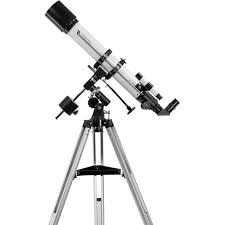
\includegraphics[scale=.4]{Ressources/TSPE_C13_AE_Fig1.jpeg}
		\end{minipage}
	\end{documentboxenv}
	\end{minipage}
\begin{minipage}{.43\linewidth}
		\begin{documentboxenv}{Matériel}
		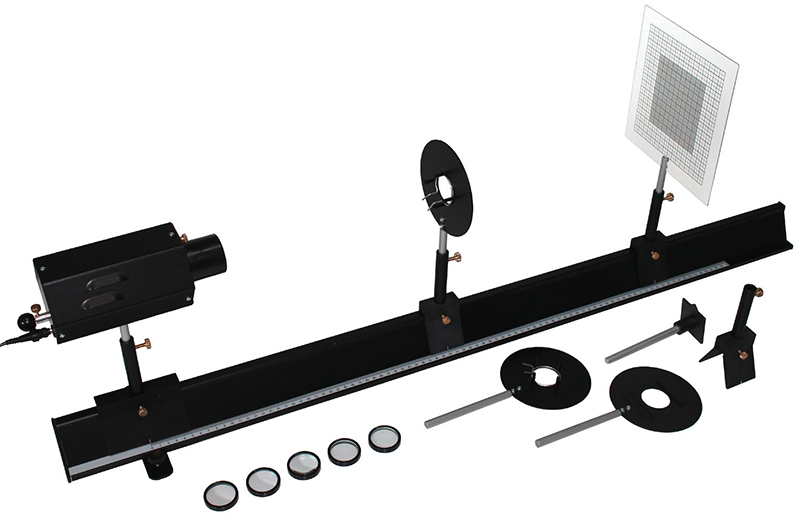
\includegraphics[width = .81\linewidth]{Ressources/TSPE_C13_AE_Fig2.jpeg}
\end{documentboxenv}
\end{minipage}

\noindent \begin{minipage}{\linewidth}
		\begin{documentboxenv}{Complément scientifique}
		Une \textbf{lunette astronomique} est modélisée par deux lentilles minces convergentes :
		\begin{itemize*}
			\item L'objectif, orienté vers l'objet lointain à observer
			\item l'oculaire, orienté vers l'\oe il de l'observateur et dont la distance focale est inférieure à celle de l'objectif.
		\end{itemize*}
	Les rayons reçus provenant d'un point objet à l'infini sont parallèles entre eux.\\
	Une lunette astronomique est dite \textbf{afocale} lorsque des rayons parallèles qui arrivent sur la lunette en ressortent parallèles entre eux. Pour cela, le foyer image $F_1'$ de l'objectif et le foyer objet $F_2$  de l'oculaire doivent être confondus, c'est-à-dire situés en une même position sur l'axe optique de la lunette.\\
	Le \textbf{grossissement} $\mathbf{G}$ d'une lunette est défini par $G=\dfrac{\theta'}{\theta}$.\\
	L'objet $AB$ situé à plusieurs mètres est vu à l'\oe il nu sous l'angle $\theta$, et l'image $A'B'$ à travers la lunette est vue sous l'angle $\theta'$ (vois schéma). L'angle $\theta$ étant petit, on admet que $\tan{\theta}=\theta$, avec $\theta$ en radian.
	\begin{center}
		\begin{tikzpicture}[scale=.95,transform shape]
			\draw[dashed,line width=1.2pt](-6,0) -- (10,0);
			\draw[Latex-Latex] (0,-3) to (0,3);
			\draw[Latex-Latex] (6.25,-3) to (6.25,3);
			\draw[dashed,line width=1.2pt](5,-3) -- (5,3);
			
			\draw[-Latex] (-6,1.5) to (6.25,-1.59); %pente = tan theta soit -0,25534
			\draw[dashed] (5,-1.2767) -- (10,3.75); %pente = tan theta' soit 1,63311
			\draw[-Latex] (6.25,-1.59) to (11.25,3.4367); %pente = tan theta' soit 1,63311
			
			\draw (0,0) node[below left]{$O_1$};
			\draw (6.25,0) node[below right]{$O_2$};
			\draw (5,2) node{$F_1'$ et $F_2$};
			
			\draw (0,3) node[above]{\textbf{Objectif}};
			\draw (6.25,3) node[above]{\textbf{Oculaire}};
			
			\draw (-6,0) node[above left]{$\leftarrow A_{\infty}$};
			\draw (-6,2) node[below left]{$\leftarrow B_{\infty}$};
			
			\draw (-5,0) node[below]{$F_1$};
			\draw (8,0) node[below]{$F'_2$};
			
			\draw (5,0) node[above left]{$A_1$};
			\draw (5,-1.2767) node[below left]{$B_1$};
			
			\draw (-2,0) arc (180:166:2) ;
			\draw (-2,.25) node[left]{$\theta$};
			
			\draw (5.5,0) arc (180:222:.75) ;
			\draw (5.6,-.25) node[left]{$\theta'$};
			
			\draw (10,0) node[above]{$\Delta$};
			
		\end{tikzpicture}
	\end{center}
\end{documentboxenv}
\end{minipage}\\

On dispose d'un objet (lettre \textbf{F} éclairée). On souhaite observer son image à travers une lunette astronomique modélisée par un rail, un écran et trois lentilles notées $\delta$ = +2, +4, +8 et +10.
\begin{enumerate}
	\item Que signifie le "+" sur les lentilles ?
	\item Calculer la distance focale de chaque lentille.
	\item Attribuer chaque lentille à $L_0$, $L_1$, $L_2$ et $L_3$. Justifier.
	\item Écrire le protocole expérimental permettant de déterminer le grossissement d'une lunette afocale à partir du matériel fourni. \textbf{APPEL n°1}
	\item Observer, avec la maquette fournie, un objet à l'infini, faire la mise au point de façon à obtenir une image nette. \textbf{APPEL n°2}
	\item Mesurer la taille de l'objet AB puis la taille de l'image A'B'. Calculer le rapport $\dfrac{A'B'}{AB}$. Conclure.
	\item Mesurer la distance entre l'objectif et l'oculaire. Calculer le grossissement de cette lunette. Conclure.
\end{enumerate}
\end{document}